%# -*- coding: utf-8-unix -*-
%%==================================================
%% test and evaluation
%%==================================================

%\bibliographystyle{sjtu2}%[此处用于每章都生产参考文献]

\chapter{系统测试与评价}
\label{chap:evaluation}
在系统软件开发中,系统测试与评价是本文关注的重点:系统的开发是否具备完整的基础功能、系统查询过程中能稳定在什么层次的性能水平,以及系统是否有足够的缺陷应对措施都是我们所需要关注的问题。

本章节主要给出系统测试文档。依据前面章节所提出的系统需求分析和系统设计实现文档,对现阶段开发的系统进行功能与性能在综合测试与评价。在测试过程中我们是主要依赖于测试原理和测试手段:测试原理主要根据系统测试理论指导,测试手段是运行系统进行实际应用查询以获取测试数据。另一方面,我们在测试过程中尽可能地模拟实际应用过程,以从用户的角度去测试系统是否具备实用性,因此系统运行环境中我们使用的数据集以实际轨迹数据为主。

\section{引言}
\label{sec:evaluation introduction}

\subsection{编写目的}
\label{subsec:purpose}
编写本章节测试与评价文档主要有以下几个目的:
\begin{itemize}
	\item 验证系统内部算法实现的正确性与可行性。
	\item 对系统产品的质量进行评价。通过对系统测试结果的数据分析以评估所设计实现的系统是否符合预期使用价值。
	\item 分析测试过程中使用的数据和信息,为之后的产品拓展提供参考资料。
	\item 分析系统产品目前阶段所存在的性能不足和使用缺陷,为下一阶段工作的提高做准备。
\end{itemize}

\subsection{针对用户}
\label{subsec:people}
\begin{itemize}
	\item 相似轨迹查询系统开发人员
	\item 相似轨迹查询系统管理人员
	\item 相似轨迹查询系统使用用户
\end{itemize}

\subsection{缺陷定义}
\label{subsec:software flaw definition}
\begin{itemize}
	\item 软件系统未实现需求分析和系统设计中的功能
	\item 软件系统未满足用户或客户的期望与需求
	\item 软件系统未满足在需求分析中预计的功能准确性与完备性。
	\item 软件测试人员难以理解系统设计而无法测试
	\item 用户个体对系统使用过程后认为系统体验不佳、系统查询效果不良。
\end{itemize}

\subsection{测试环境数据}
\label{subsec:environment}

\subsubsection{测试数据集}
\label{subsubsec:dataset}
上海私家车OBD轨迹数据集\cite{NRL}。其中有三种数据格式的数据。在系统测试中,我们选择数据定义为GPS\_routine\_3的第三种数据类型私家车轨迹数据,如表\ref{tab-gpsroutine3}所示:
	\begin{table}[!htpb]
  	\centering
		\begin{tabular}{ |p{2cm}|p{3.5cm}|p{2cm}|p{4.5cm}| }
		\hline
		字段名称 & 含义 & 类型 & 备注\\
		\hline
		id & 记录号 & & 自增id \\
		\hline
		obd\_id & obd设备号 & String & \\
		\hline
		经纬度 & 地理坐标 &  & \\
		\hline
		obd端时间 & & 时间 & yyyy-mm-dd 时分秒\\
		\hline
		车辆状态 & 速度、发动机转速 & & \\
		\hline 
		\end{tabular}
		\bicaption[tab-gpsroutine3]{系统测试选取轨迹数据格式}{系统测试选取轨迹数据格式}{Table}{A list of data fields of private trajectory data}
	\end{table}
	
	本文选择其中时间范围为2015年4月份的轨迹数据。原始轨迹数据的一条数据包含表\ref{tab-gpsroutine3}的中所有的字段值,其中数据项目以时间顺序依次存储。系统处理过程中,假设在第三种数据结构下,如果一个obd用户的两个坐标点时间间隔超过半个小时,则两个坐标点属于不同的两天轨迹数据。基于这一假设,系统在预处理阶段轨将每个用户的轨迹点划分到对应的轨迹数据中,生成用户的轨迹历史数据。
	
\begin{figure}[!htp]
  \centering
  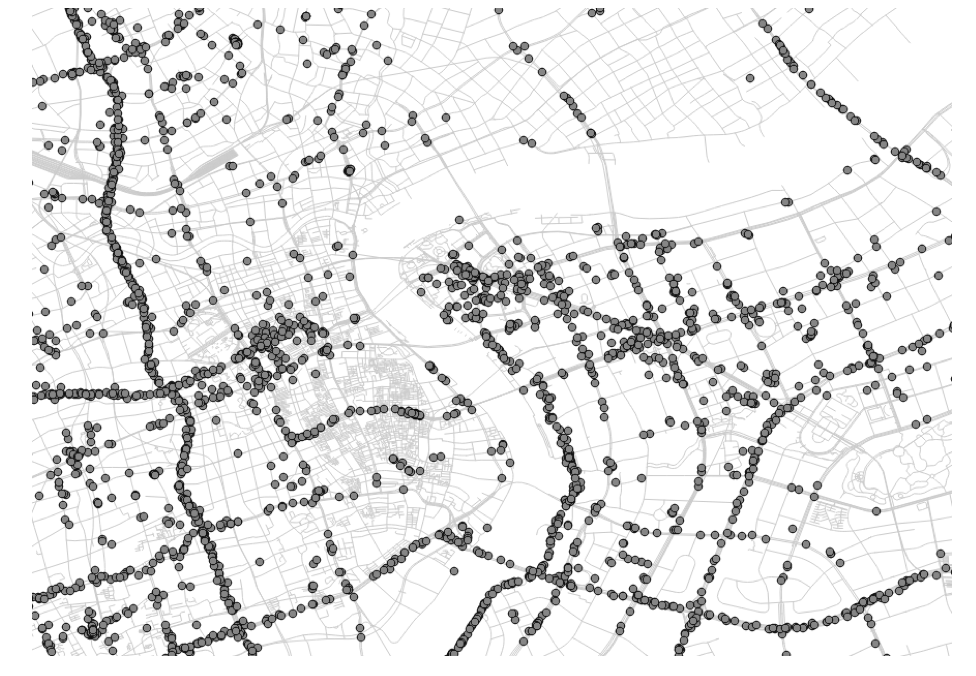
\includegraphics[width=0.5\textwidth]{evaluation/obd.png}
  \bicaption[fig:obd data]{上海市私家车轨迹数据样例}{上海市私家车轨迹数据样例\cite{NRL}}{Fig}{An example of Shanghai OBD private trajectories data}
\end{figure}


\subsubsection{测试设备环境}
\label{subsubsec:device}
\begin{enumerate}
	\item 单机测试环境
	\begin{itemize}
		\item Mac OS X EI Caption操作系统
		\item 2.6 GHz Intel Core i5处理器
		\item 8GB 1600 MHz DDR3内存
	\end{itemize}
	\item 分布式集群处理环境
	\begin{itemize}
		\item Ubuntu14.04 amd64操作系统
		\item 2.6 GHz Intel Core i5处理器
		\item 1GB DDR3内存
	\end{itemize}
\end{enumerate}

\section{系统测试概要}
\label{sec:general description}
本章节大体从系统的功能和性能两个方面入手对本文所设计并实现的相似轨迹查询系统进行测试。在功能测试方面,测试主要的目的在于考察系统实现是否完成需求分析与系统设计中的预期功能,保证用户在使用系统过程中能够正常使用任一一个系统的子功能从而保证用户使用系统的流畅性与完整性;在性能测试方面,测试主要的目的在于分析系统实现是否能够高效并准确地为用户提供查询结果或是其他交互方面为用户提供良好的使用体验,在网页系统中,良好的交互性与结果的准确性是一个系统在用户群中不断使用的根本保证。

\section{系统测试描述}
\label{sec:function test}

\subsection{功能测试描述}
\label{subsec:function test description}
本文所设计的功能测试中的各类操作主要针对组成相似轨迹查询系统的的单一功能模块,每个操作步骤对应的就是一个功能点,即功能模块。由于本文所设计的相似轨迹查询系统由用户模块和管理员模块两个大部分组成,因此我们需要再分别对两个主要模块内部的功能模块进行系统使用测试。

\subsection{性能测试描述}
\label{subsec:performance test description}
在单机测试环境中,本文所设计的性能测试主要是位了获取系统在各种应用或者不同输入参数的情况下对查询效率和查询准确的反应情况。由于该系统的主要针对群里是用户对象,因此性能是本次测试中的重点考虑因素,一个良好的系统应该能够给予用户较好的交互体验。由于系统设计与实现并不一定合理,本文尽可能的考虑系统在查询过程中的上限性能,找出在现阶段中系统可能仍然存在的不足或亟待改善的部分,为今后系统的拓展和升级提供参考思路。

对于分布式性能的测试,由于系统设备限制问题,本文在本次测试中仅给出在分布式环境在系统完成任务时所需要的查询时间。我们在测试中证明对于分布式,在对于目前查询性能影响较大的时间因子在于读取HDFS文件系统中。也将相似轨迹查询在分布式集群处理环境下的性能提高目标放在今后系统能够运行在更优秀的集群环境中。

\section{系统测评结果}
\label{sec:test result}

\subsection{功能测试结果}
\label{subsec:function test result}

\subsection{性能测试结果}
\label{subsec:performance test result}

在性能测试方面,对于单机测试本文设定一下测试条件
\begin{itemize}
	\item 测试变量:相似轨迹查询数目和查询位置点数目。
	\item 测试指标:相似轨迹查询时间和查询准确度。
	\item 测试类型:相似轨迹无序查询和有序查询。
\end{itemize}

\begin{figure}[!htp]
  \centering
  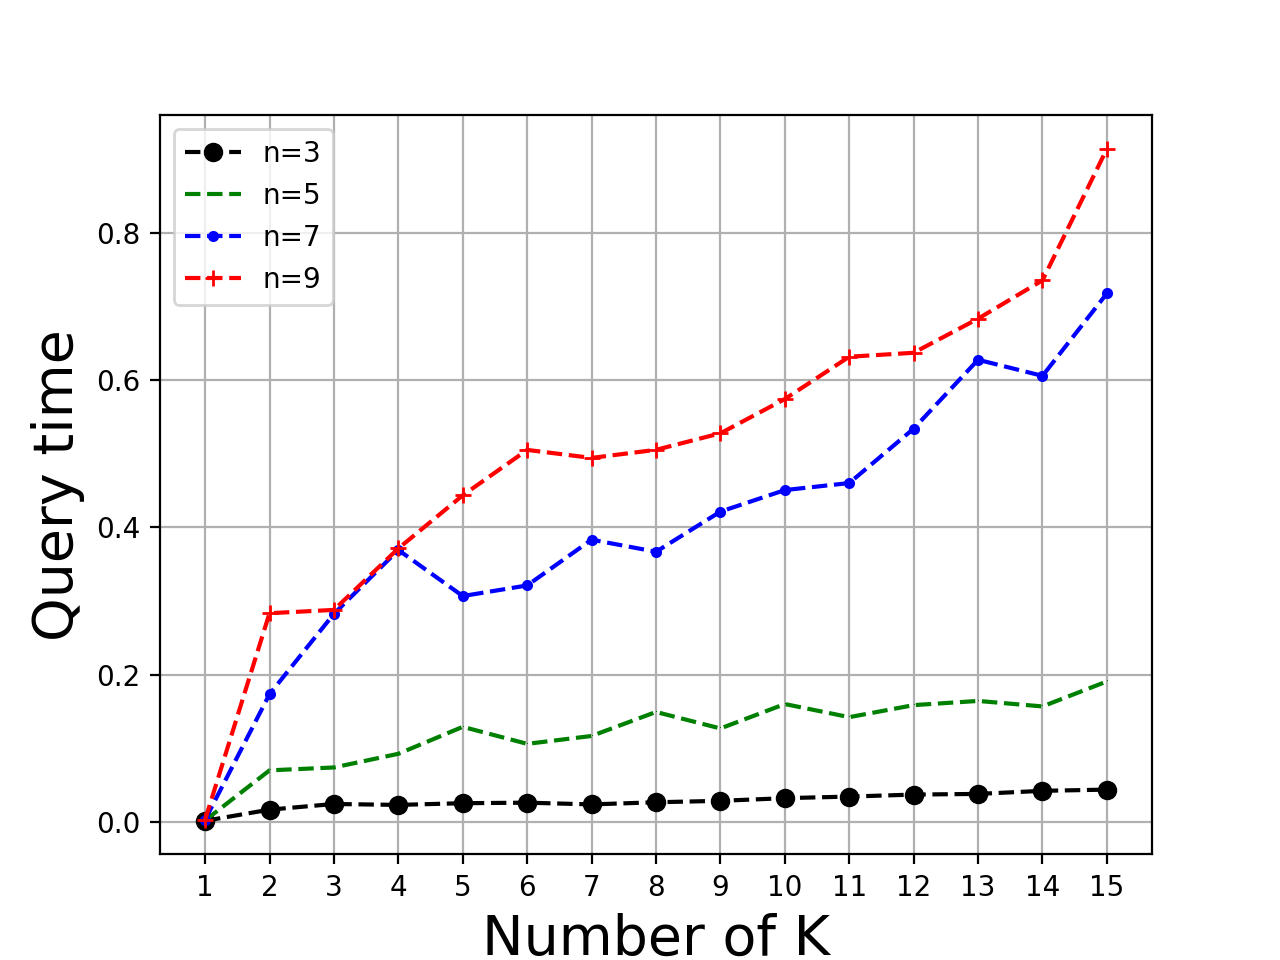
\includegraphics[width=0.45\textwidth]{evaluation/figure1.png}
  \hspace{0.5cm}
  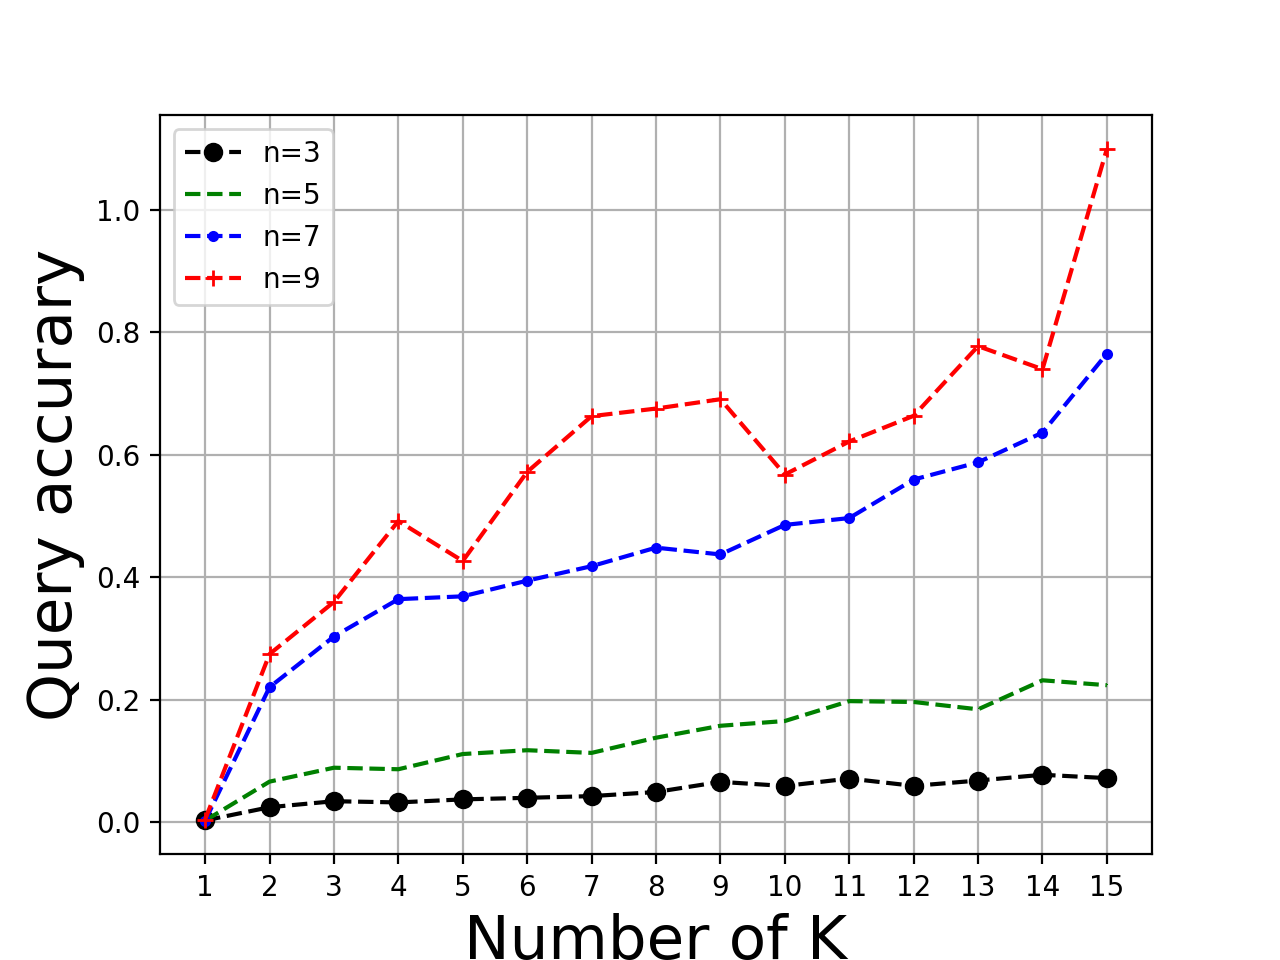
\includegraphics[width=0.45\textwidth]{evaluation/figure2.png}
  \bicaption[fig:number k-time]{相似轨迹查询数目k和查询时间的关系}{相似轨迹查询数目k和查询时间的关系(左图无序查询,有图有序查询)}{Fig}{Query time for the number of k trajectories}
\end{figure}

\begin{figure}[!htp]
  \centering
  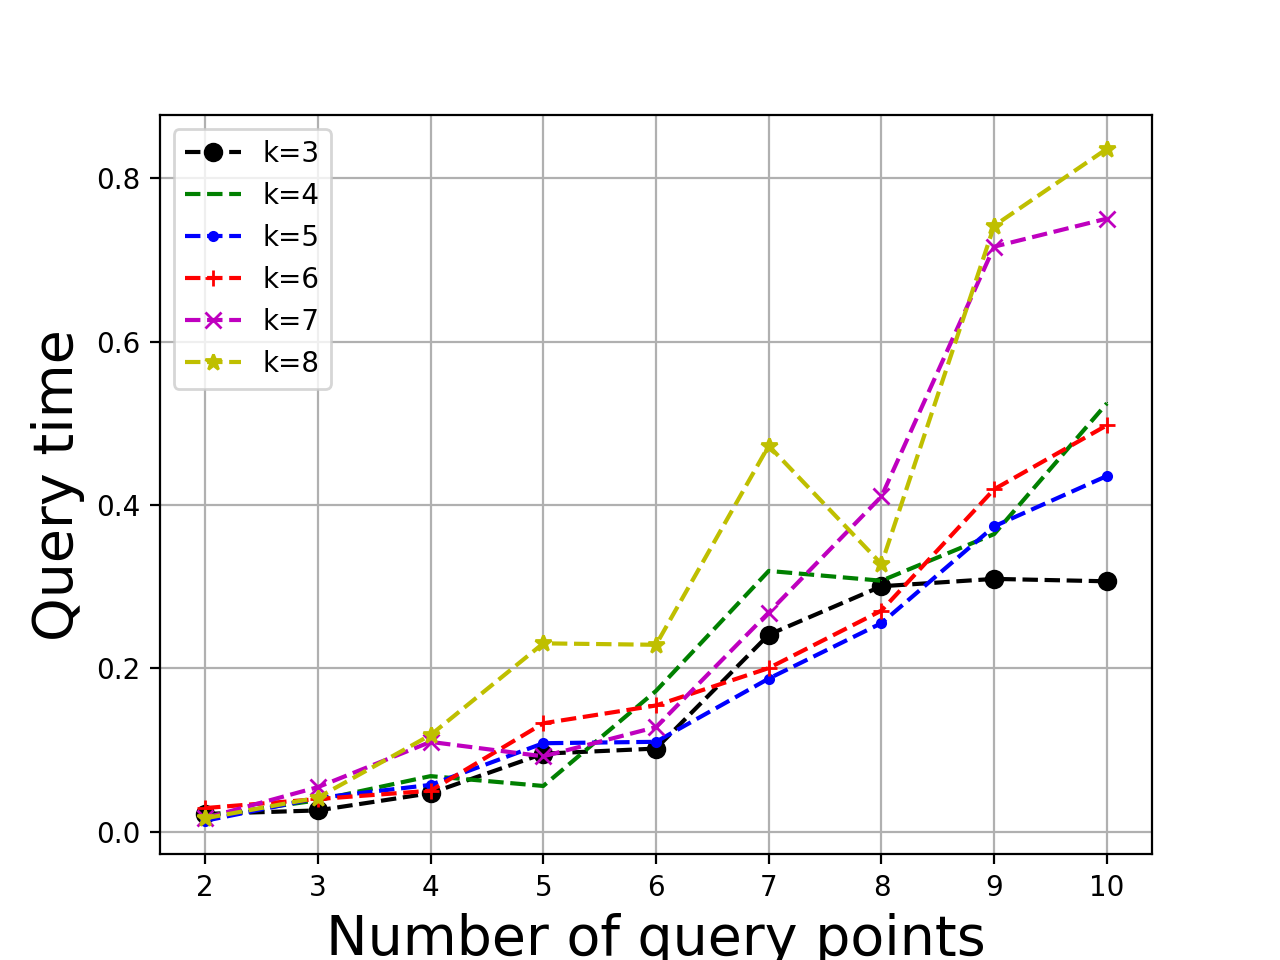
\includegraphics[width=0.45\textwidth]{evaluation/figure3.png}
  \hspace{0.5cm}
  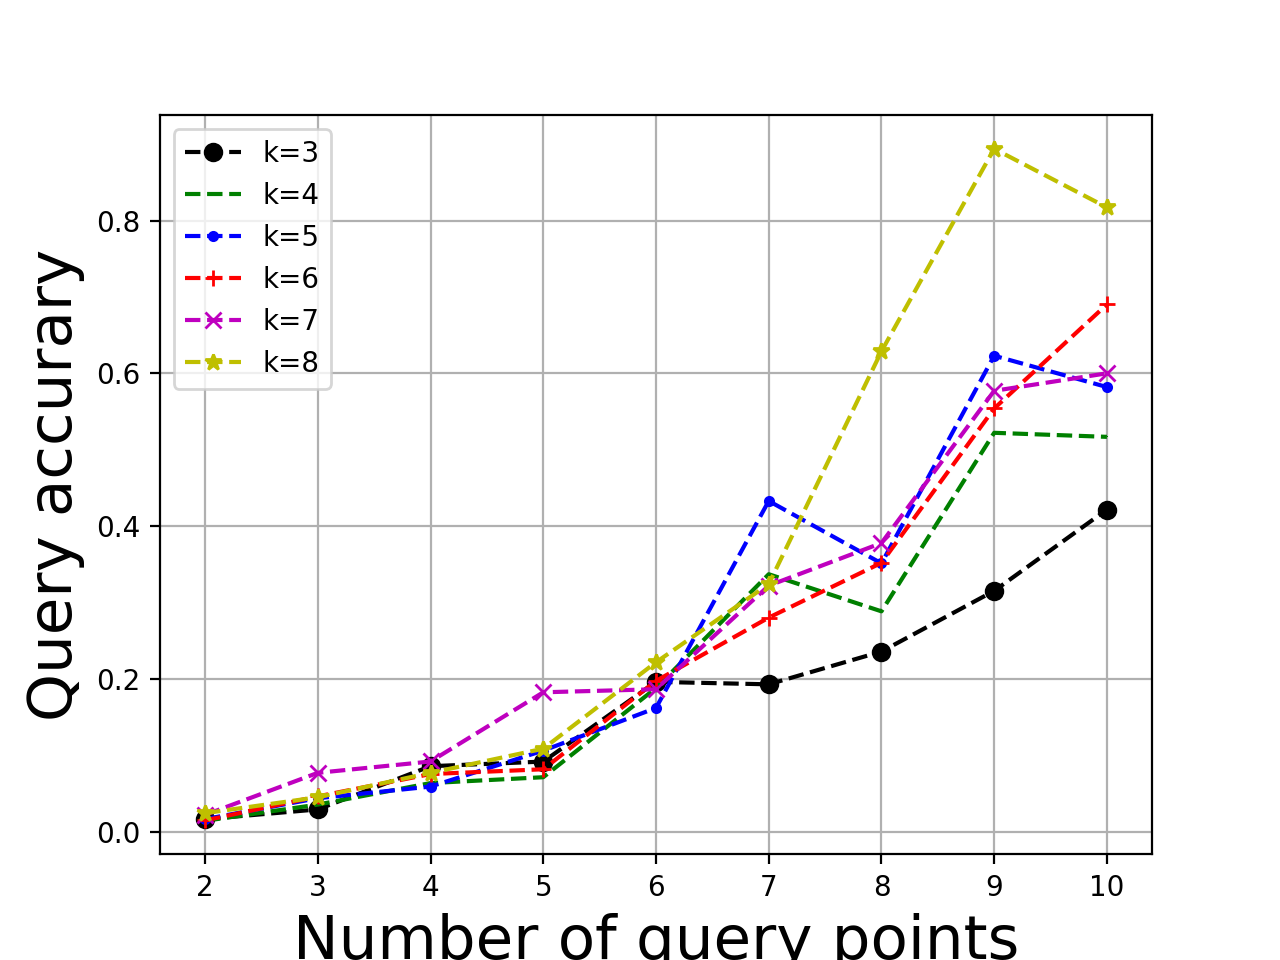
\includegraphics[width=0.45\textwidth]{evaluation/figure4.png}
  \bicaption[fig:number of querypoint-time]{相似轨迹查询点数目和查询时间的关系}{相似轨迹查询点数目和查询时间的关系(左图无序查询,有图有序查询)}{Fig}{Query time for the number of query points}
\end{figure}

\begin{figure}[!htp]
  \centering
  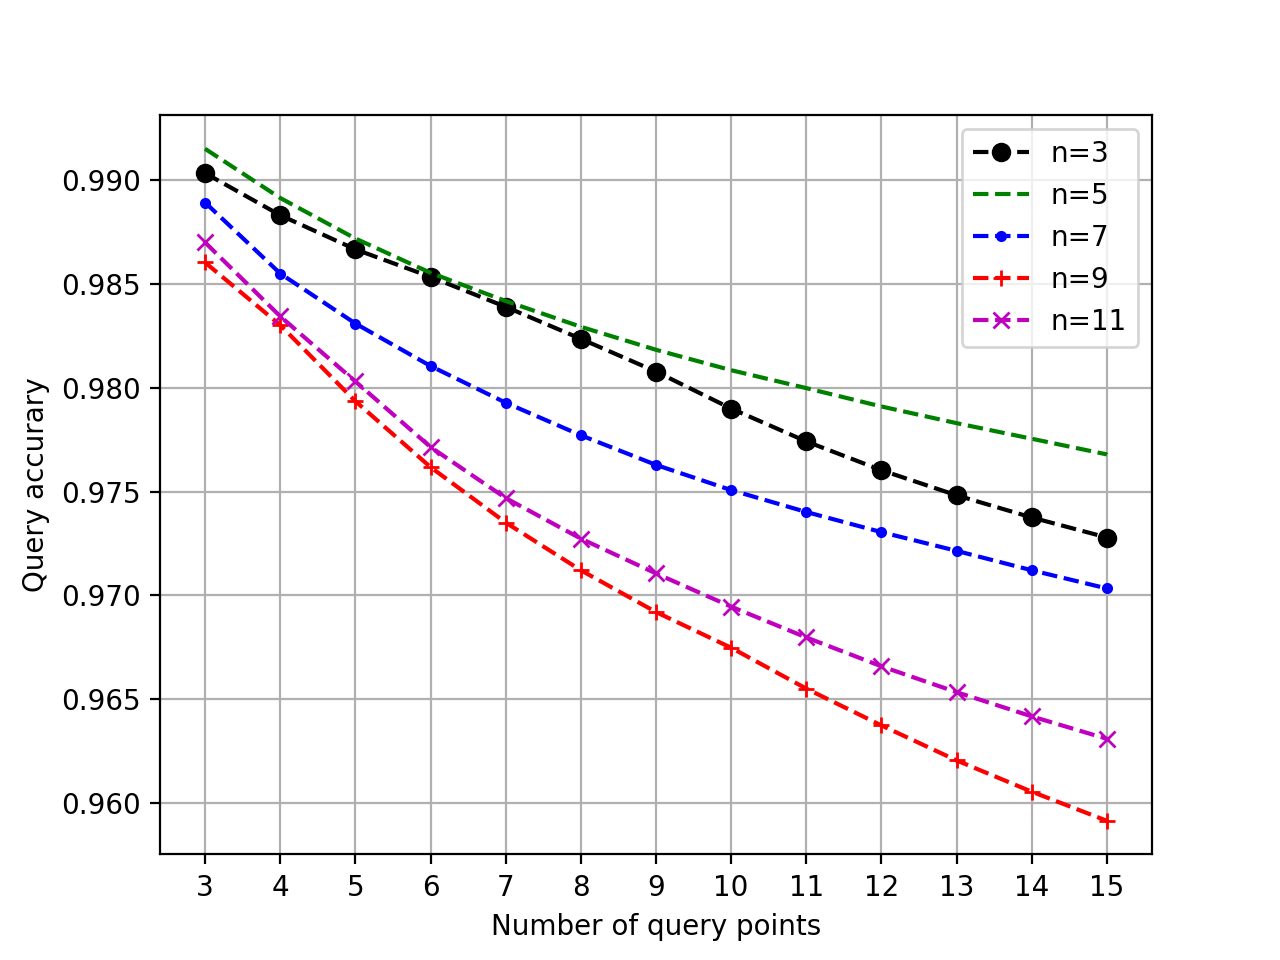
\includegraphics[width=0.45\textwidth]{evaluation/figure5.png}
  \hspace{0.5cm}
  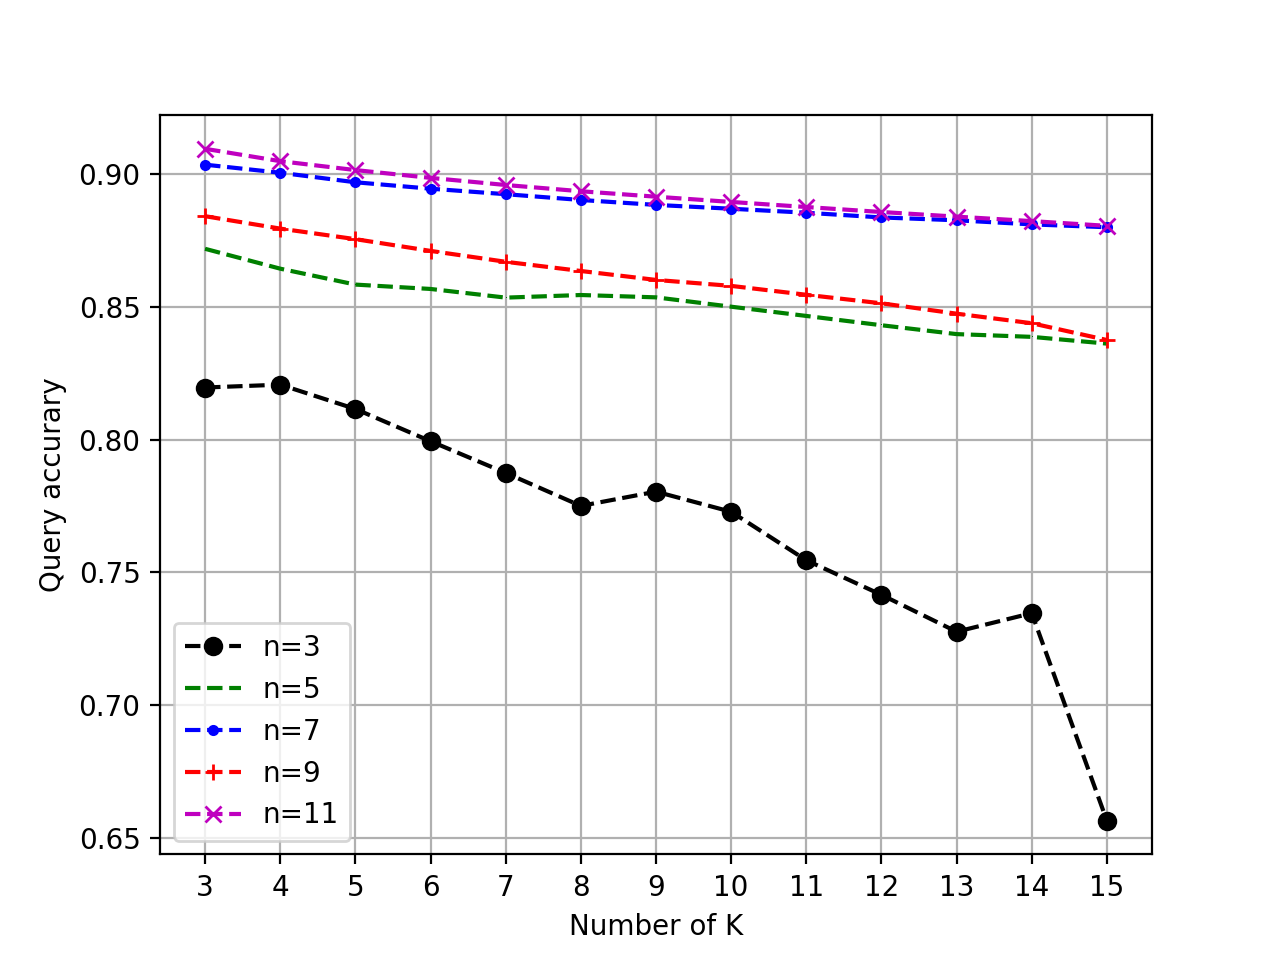
\includegraphics[width=0.45\textwidth]{evaluation/figure6.png}
  \bicaption[fig:number k-accuracy]{相似轨迹查询数目k和查询准确度的关系}{相似轨迹查询数目k和查询准确度的关系(左图无序查询,有图有序查询)}{Fig}{Query accuracy for the number of k trajectories}
\end{figure}

\begin{figure}[!htp]
  \centering
  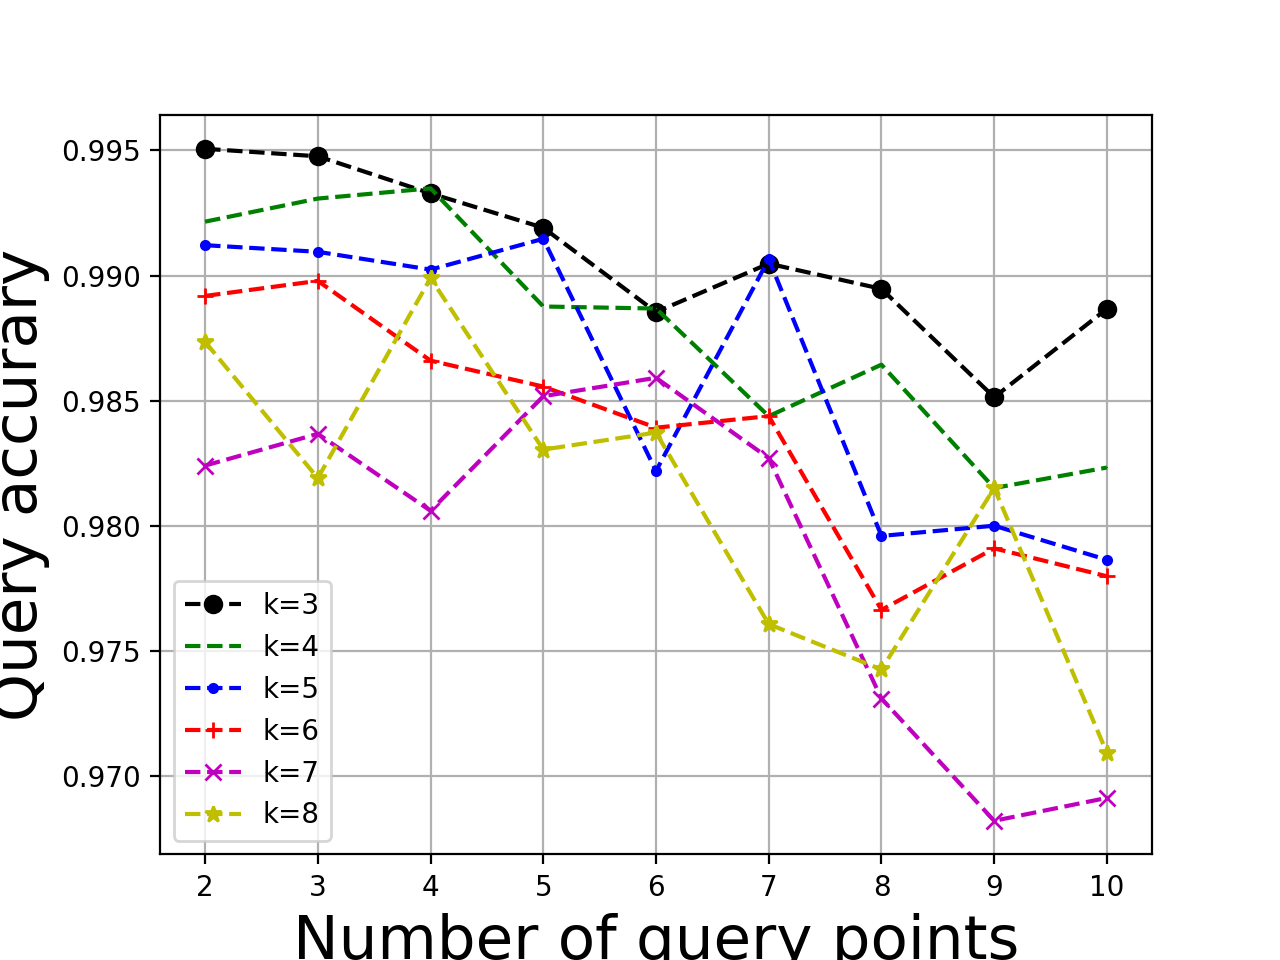
\includegraphics[width=0.45\textwidth]{evaluation/figure7.png}
  \hspace{0.5cm}
  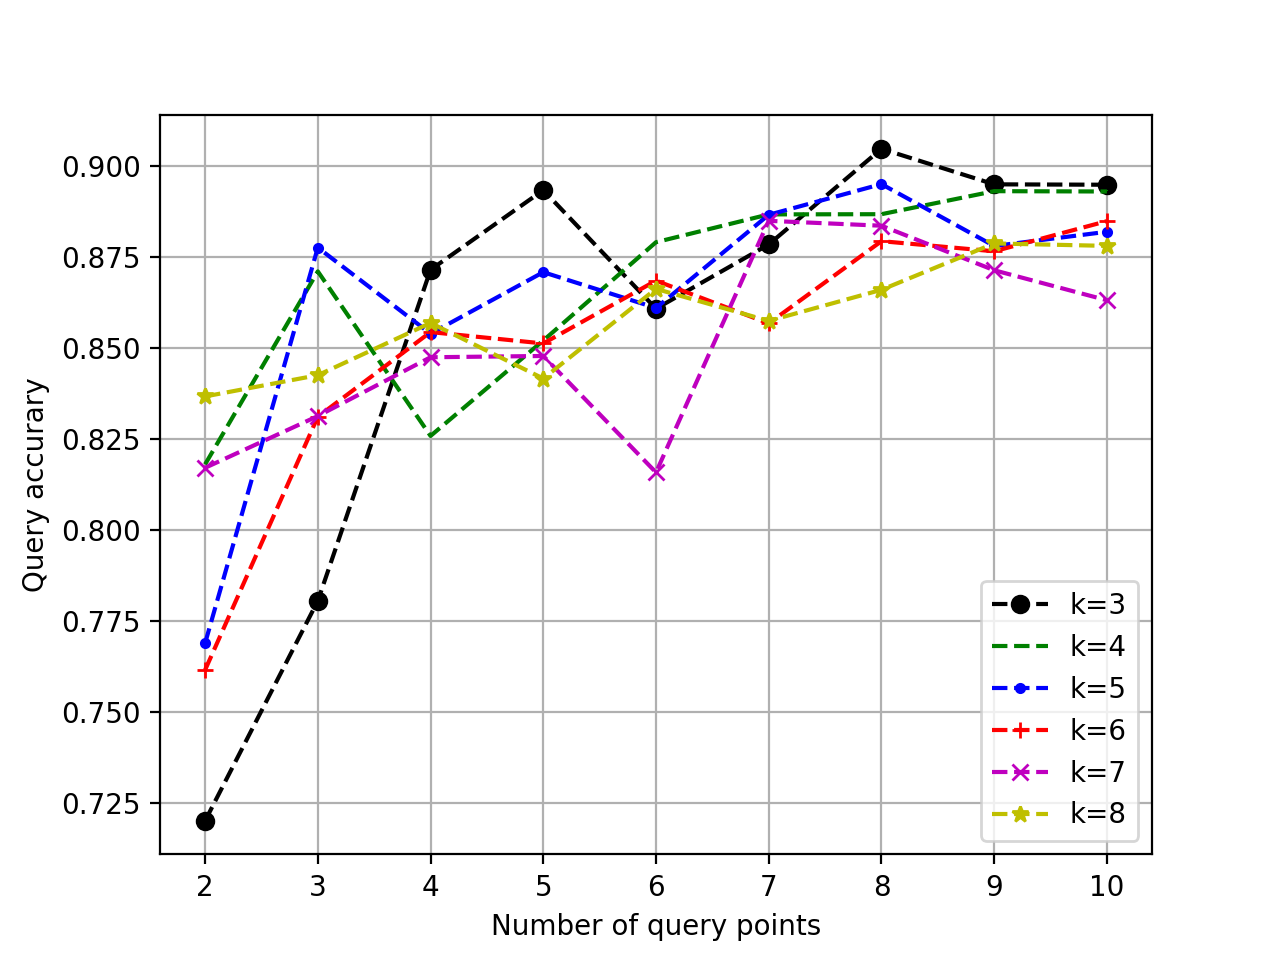
\includegraphics[width=0.45\textwidth]{evaluation/figure8.png}
  \bicaption[fig:number k-accuracy]{相似轨迹查询点数目和查询准确度的关系}{相似轨迹查询点数目和查询准确度的关系(左图无序查询,有图有序查询)}{Fig}{Query accuracy for the number of query points}
\end{figure}

\section{系统测试评价}
\label{sec:system evaluation}
根据上述的测试结果,本文从测试结果所对应的功能和性能两个方面对相似轨迹查询系统做出客观评价。
\begin{itemize}
	\item 从系统功能方面,相似轨迹查询系统完成了以用户为主体对象的用户模块和一部分管理模块功能,初步完成了一个面向用户群里的相似轨迹查询,在必要功能组成上具备完整性。不过功能组成相对简单,在之后基于现阶段的系统设计与实现任务中,应该更多地结合实际应用以丰富完整系统的功能组成。
	\item 从系统性能方面,从测试结果提供的查询时间折线图可以观察得出结论:系统较好地实现了内部的算法部分,单机环境查询结果具有高效性和准确性,能够在大部分实际应用中给予用户良好的查询体验。
	\item 测试过程中也发现了一些不足之处:功能组成相对简单,在之后基于现阶段的系统设计与实现任务中,应该更多地结合实际应用以丰富完整系统的功能组成;性能测试阶段也反应出在测试过程中存在一些误差点,这些误差产生的主要原因主要是由于数据集轨迹较大导致其中中一些噪音点没有预先除去,在之后的测试中应当予以注意。
\end{itemize}

\section{本章小结}
\label{sec:evaluation conclusion}
本章节主要对本文根据相似轨迹查询算法所设计并实现的相似轨迹查询系统进行测试和评价。在测试过程中,参考了目前对软件系统测试的基本方法和理论指导,从功能和性能两个主要方面入手对系统展开测试并得出基本结果。基于这一结果,本文再对系统本文进行评价操作,以符合实际情况。

